\documentclass[xcolor=table]{beamer}
\usetheme{boxes}

\usepackage[utf8]{inputenc}
\usepackage[T1]{fontenc}
\usepackage[brazil]{babel}
\usepackage{amsmath}
\usepackage{amsfonts}
\usepackage{amssymb}
\usepackage{graphicx}
\usepackage{booktabs}
\usepackage{adjustbox}
\usepackage{multirow}

\author{Bruno Ferrari Guide}
\title{Abordagem computacional para a questão do acento no português brasileiro}
\subtitle{III WORKSHOP DE LINGUÍSTICA COMPUTACIONAL}
%\logo{}
\institute{Orientador: Marcelo Barra Ferreira\\ Departamento de Linguística - FFLCH - USP}
\date{8 de dezembro de 2016}
%\subject{}
%\setbeamercovered{transparent}
%\setbeamertemplate{navigation symbols}{}

\begin{document}
	%1
	\maketitle
%%%%%%%%%%%%%%%%%%%%%%%%%%%%%%%%%%%%%%%%%%
	\section{Introdução}
	%2
	\begin{frame}
		\frametitle{Introdução}
		\begin{itemize}
			\item Tópicos dessa apresentação:\\
			\begin{itemize}
				\item Objetivos\\
				\item Resumo\\
				\item Resultados\\
			\end{itemize}
		\end{itemize}
	\end{frame}

%%%%%%%%%%%%%%%%%%%%%%%%%%%%%%%%%%%%%%%%%%%%%

	\section{Objetivos}
	%3
	\begin{frame}
		\frametitle{Objetivos do projeto}
		\begin{itemize}
			\item Revisar abordagens para a questão do acento.\\
			\item A partir de dados coletados do idioma, apresentar uma análise quantitativa sobre o comportamento do acento em relação a algumas variáveis linguísticas.\\
			\item Implementar modelos computacionais preditivos do acento para fundamentar uma discussão sobre o tema.\\
		\end{itemize}
	\end{frame}


%%%%%%%%%%%%%%%%%%%%%%%%%%%%%%%%%%%%%%%%%%%%%

	\section{Resumo}
	\begin{frame}
		\frametitle{Sobre o Acento - 2 tendências}
		\begin{itemize}
			\item O acento no português brasileiro (quase) sempre ocupa uma das três últimas posições da palavra, criando as três categorias acentuais: Oxítona, Paroxítona, Proparoxítona.
			\item Duas tendências dão conta da maioria das palavras do PB:
			\begin{itemize}
				\item Caso a sílaba final seja pesada, a palavra é oxítona.\\
				\item Caso a sílaba final seja leve, a palavra é paroxítona.\\
			\end{itemize}
		\end{itemize}
	\end{frame}
	%5
	\begin{frame}
		\frametitle{2 tendências?}
		\begin{itemize}
			\item Problemas com palavras oxítonas terminadas em sílaba leve, como \textit{caqui, urubu}\\
			\item Problemas com paroxítonas terminadas em sílaba pesada, como em \textit{mártir, câncer, difícil}.\\
			\item Problemas com as proparoxítonas de modo geral.\\
			\item O acento é regular, porém tem irregularidades.\\
			\item O acento é irregular, porém tem regularidades.\\
		\end{itemize}

	\end{frame}	
%%%%%%%%%%%%%%%%%%%%%%%%%%%%%%%%%%%%%%%%%%%%%%%%%%%%%

	\begin{frame}
		\frametitle{Sobre modelos probabilísticos}
		\begin{itemize}
			\item Modelo é uma representação formal de um objeto.\\
			\item As vezes, o objeto possui comportamento imprevisível.\\
			\item Na matemática, a área que lida com a imprevisibilidade (ou seja, que a quantifica e formaliza) é a probabilidade.\\
			\item Existem muitas formas de tentar formalizar essa imprevisibilidade, cada uma possui suas vantagens e desvantagens.\\
		\end{itemize}
	\end{frame}
	
	\begin{frame}
		\frametitle{Modelos implementados e Propostas analisadas}
		\begin{itemize}
			\item Propostas analisadas:\\
			\begin{itemize}
				\item Bisol (1992)\\
				\item Lee (1995)\\
			\end{itemize}
			\item Modelos probabilísticos:\\
			\begin{itemize}
				\item N-gramas\\
				\item Classificador Bayesiano Ingênuo\\
			\end{itemize}
			\item Modelo arbitrário:
			\begin{itemize}
				\item \textit{Baseline}\\
			\end{itemize}			
		\end{itemize}
	\end{frame}
	\begin{frame}
		\frametitle{Análise das propostas e definição de baseline}
		\begin{itemize}
			\item Bisol (1992)\\
			\begin{itemize}
				\item Se a palavra termina em sílaba pesada, é oxítona.\\
				\item Senão, é paroxítona.\\
			\end{itemize}
			\item Lee (1995)\\
			\begin{itemize}
				\item Não-verbos: Oxítonas com sílaba final leve ou pesada são previstas. Paroxítonas com sílaba final leve também.\\
				\item Verbos: Paroxítonas terminadas em sílaba leve e oxítonas terminadas em sílaba pesada são previstas.
			\end{itemize}
			\item \textit{Baseline}\\
			\begin{itemize}
				\item Toda palavra é paroxítona.\\
			\end{itemize}
		\end{itemize}
	\end{frame}
	\begin{frame}
		\frametitle{Exemplo: N-gramas}
		\begin{itemize}
			\item Palavra: 'casa'\\
			\item Representação: '\&ka-za*'\\
			\item Probabilidade obtida a partir do cálculo:\\
			\begin{itemize}
				\item BIGRAMAS P('\&ka-za*') = P('\&k') $\times$ P('ka') $\times$ P('a-') $\times$ P('-z') $\times$ P('za') $\times$ P('a*')\\
				\item TRIGRAMAS P('\&ka-za*') = P('\&ka') $\times$ P('ka-') $\times$ P('a-z') $\times$ P('-za') $\times$ P('za*')\\
			\end{itemize} 

		\end{itemize}
	\end{frame}
	\begin{frame}
		\frametitle{Exemplo: Classificador Bayesiano Ingênuo}
		\begin{itemize}
			\item Palavra: 'perna'\\
			\item Vetor de traços: [Categoria morfossintática: 'Nome', estrutura silábica: 'CVC-CV', nivel de frequência no corpus: 3]\\
			\item Probabilidades:
			\begin{itemize}
				\item Oxítona = p(oxítona)* p('nome'|oxítona) * p('leve'|oxítona)...
				\item Paroxítona = p(paroxítona)* p('nome'|paroxítona) * p('leve'|paroxítona)...
				\item Proparoxítona = p(proparoxítona)* p('nome'|proparoxítona) * p('leve'|proparoxítona)...
			\end{itemize}
			\item Repare que os meus \textit{priors} vão favorecer as categorias paroxítona, oxítona e proparoxítona nessa ordem.\\
			
		\end{itemize}	
	\end{frame}
	
	\begin{frame}
		\frametitle{Implementação}
		\begin{itemize}
			\item Corpus utilizado: ABG $\rightarrow$ 98.000 palavras.\\
			\item Implementação feita em Python.\\
			\item Foi efeituada uma \textit{Cross-validation} dos resultados.\\
			\item Acertos e erros em comparação com acentuação categórica já presente no corpus.\\
		\end{itemize}
	\end{frame}

%%%%%%%%%%%%%%%%%%%%%%%%%%%%%%%%%%%%%%%%%%%%%%
	\section{Resultados}
	\begin{frame}

		\centering \textbf{Resultados}
	\end{frame}
	
	\begin{frame}
		\frametitle{Desempenho do modelo baseado em Bisol(1992) para os verbos}
\begin{table}[H]
	\centering
	\label{TAB27}
	\begin{tabular}{@{}lccr@{}}
		\toprule
		\textbf{Bisol (1992)}          & \textbf{\% de tipos}   & \textbf{\% de ocorrências} & \textbf{Acerto} \\ \midrule
		Verbos                & 48,60       & 33,12           &        \\
		Oxítonas leves                & 15,31       & 23,20           & Não      \\
		\rowcolor[HTML]{656565} 
		Oxítonas pesadas                & 24,99       & 32,97           & Sim      \\
		\rowcolor[HTML]{656565} 
		Paroxítonas leves               & 58,10       & 42,48           & Sim      \\
		Paroxítonas pesadas               & 1,26        & 1,27            & Não      \\
		Proparoxítonas leves                & 0,33        & 0,06            & Não      \\
		Proparoxítonas pesadas                & 0,00        & 0,01            & Não      \\
		\% Acerto verbos           & 83,09       & 75,45           &        \\
		\% do total           & 40,38       & 24,99           &        \\
		&               &                   &        \\
	
	\end{tabular}
\end{table}


	\end{frame}
	
	\begin{frame}
		\frametitle{Desempenho do modelo baseado em Lee (1995) para os verbos}
		\begin{table}[H]
			\centering
			\label{TAB28}
			\begin{tabular}{@{}lccr@{}}
				\toprule
				\textbf{Lee (1995)}            &\textbf{ \% de tipos}   & \textbf{\% de ocorrências} & \textbf{Acerto} \\ \midrule
				Verbos                & 48,60       & 33,12           &        \\
				Oxítonas leves                & 15,31       & 23,20           & Não      \\
				Oxítonas pesadas                & 24,99       & 32,97           & Não      \\
				\rowcolor[HTML]{656565} 
				Paroxítonas leves               & 58,10       & 42,48           & Sim      \\
				\rowcolor[HTML]{656565} 
				Paroxítonas pesadas               & 1,26        & 1,27            & Sim      \\
				Proparoxítonas leves                & 0,33        & 0,06            & Não      \\
				Proparoxítonas pesadas                & 0,00        & 0,01            & Não      \\
				\% Acerto verbos          & 59,36       & 43,75           &        \\
				\% do total           & 28,85       & 14,49           &        \\
			\end{tabular}
		\end{table}
	\end{frame}
	\begin{frame}
	\frametitle{Desempenho do modelo baseado em Bisol (1992) para os não-verbos}
\begin{table}[H]
	\centering
	\label{TAB227}
	\begin{tabular}{@{}lccr@{}}
		\toprule
		\textbf{Bisol (1992)}          & \textbf{\% de tipos}   & \textbf{\% de ocorrências} & \textbf{Acerto} \\ \midrule
			Não-verbos            & 51,40       & 66,88           &        \\
			Oxítonas leves                & 10,01       & 4,78            & Não      \\
			\rowcolor[HTML]{656565} 
			Oxítonas pesadas                & 8,76        & 23,48           & Sim      \\
			\rowcolor[HTML]{656565} 
			Paroxítonas leves               & 68,51       & 66,25           & Sim      \\
			Paroxítonas pesadas               & 4,98        & 1,41            & Não      \\
			Proparoxítonas leves                & 7,46        & 3,64            & Não      \\
			Proparoxítonas pesadas                & 0,28        & 0,44            & Não      \\
			\% Acerto não-verbos          & 77,27       & 89,73           &        \\
			\% do total           & 39,72       & 60,01           &        \\
			&               &                   &        \\
			{\bf \% Acerto total} & {\bf 80,10} & {\bf 85,00}     & {\bf } \\ \bottomrule
			\end{tabular}
		\end{table}

	\end{frame}
	
	\begin{frame}
		\frametitle{Desempenho do modelo baseado em Lee (1995) para os não-verbos}
		\begin{table}[H]
			\centering
			\label{TAB29}
			\begin{tabular}{@{}lccr@{}}
				\toprule
				\textbf{Lee (1995)}            &\textbf{ \% de tipos}   & \textbf{\% de ocorrências} & \textbf{Acerto} \\ \midrule
			Não-verbos            & 51,40       & 66,88           &        \\
			\rowcolor[HTML]{656565} 
			Oxítonas leves                & 10,01       & 4,78            & Sim      \\
			\rowcolor[HTML]{656565} 
			Oxítonas pesadas                & 8,76        & 23,48           & Sim      \\
			\rowcolor[HTML]{656565} 
			Paroxítonas leves               & 68,51       & 66,25           & Sim      \\
			Paroxítonas pesadas               & 4,98        & 1,41            & Não      \\
			Proparoxítonas leves                & 7,46        & 3,64            & Não      \\
			Proparoxítonas pesadas                & 0,28        & 0,44            & Não      \\
			\% Acerto não-verbos         & 87,28       & 94,51           &        \\
			\% do total           & 44,86       & 63,21           &        \\
			&               &                   &        \\
			{\bf \% Acerto total} & {\bf 73,71} & {\bf 77,70}     & {\bf } \\ \bottomrule
				\end{tabular}
			\end{table}
	\end{frame}
	
	\begin{frame}
		\frametitle{Resultados: N-gramas}
		\begin{figure}
\centering
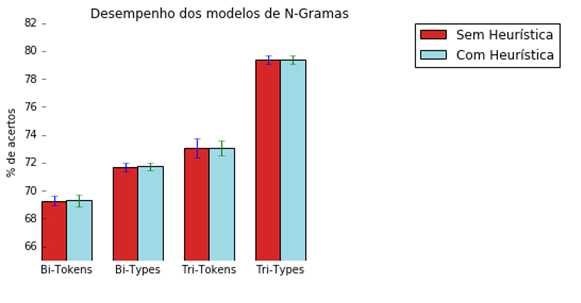
\includegraphics[width=0.7\linewidth]{graf-ngramas1}
\label{fig:graf-ngramas1}
\end{figure}

	\end{frame}

	\begin{frame}
		\frametitle{Resultados: N-gramas Sílabas}
		\begin{figure}
\centering
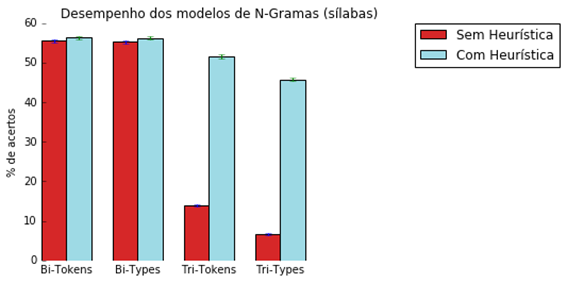
\includegraphics[width=0.7\linewidth]{graf-ngramas-sil}
\label{fig:graf-ngramas-sil}
\end{figure}

	\end{frame}	
	\begin{frame}
		\frametitle{Resultados: CBI}
		\begin{itemize}

			\item N = Nível de frequência\\
			\item C = Categoria Morfossintática\\
			\item E = Estrutura silábica (CV-CV)\\
		\end{itemize}
	\end{frame}
	
%	\begin{frame}
%		\frametitle{Resutlados CBI}
%		\begin{figure}
%\centering
%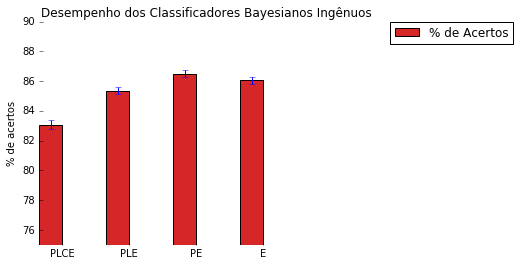
\includegraphics[width=0.9\linewidth]{resultadosnbc}
%\label{fig:resultadosnbc}
%\end{figure}

%	\end{frame}
	\begin{frame}
		\frametitle{Tabela: CBI}
		\begin{table}[]
			\centering
			\label{TAB44}
			\caption{Desempenho dos classificadores bayesianos ingênuos montados a partir de diferentes subconjuntos de variáveis.}
			\begin{tabular}{@{}lcr@{}}
				
				\textbf{Nome}  & \textbf{Média} & \textbf{Desvio} \\ \midrule
				E              & 91,93          & 0,20            \\
				CE             & 90,18          & 0,22            \\
				EN             & 90,09          & 0,22            \\
				CEN            & 86,45          & 0,26            \\
				N              & 66,64          & 0,36            \\
				CN             & 66,62          & 0,35            \\
				C              & 66,59          & 0,33            \\
			\end{tabular}
		\end{table}
	\end{frame}
	\begin{frame}
		\frametitle{Resultados: Geral}
		\begin{figure}
\centering
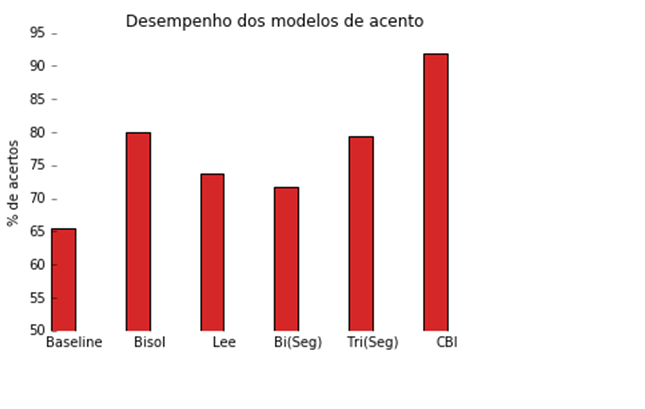
\includegraphics[width=0.9\linewidth]{graf-cbigeral}
\label{fig:graf-cbigeral}
\end{figure}

	\end{frame}
	\begin{frame}
		\frametitle{Tabela: Desempenho geral}
		\begin{table}[]
			\centering
			\caption{Desempenho Geral}
			\label{my-label}
			\begin{tabular}{@{}ll@{}}
				\toprule
				Parâmetros & Média \\ \midrule
				CBI E    & 91.93 \\
				Bisol      & 80.10 \\
				Trigramas  & 79.40 \\
				Lee        & 73.71 \\
				Bigramas   & 71.69 \\
				Baseline   & 65.59 \\ \bottomrule
			\end{tabular}
		\end{table}
	\end{frame}
	
	
	\begin{frame}
		\frametitle{Conclusões}
		\begin{itemize}
			\item Após as análises feitas, a marcação arbitrária para descrever o comportamento do acento no PB não pôde ser descartada. Mas o funcionamento da marcação arbitrária para a previsão do acento não é uma questão trivial.\\
			\item O peso da sílaba final é a variável linguística estudada que mais possui relação estatística com o comportamento do acento.\\
			\item A melhoria do modelo baseado em trigramas quando comparado com o modelo de bigramas sugere que há motivos para se conduzir uma nova análise usando modelos baseados em tetragramas.\\
			\item O CBI que se vale da probabilidade da estrutura silábica da palavra pertencer a uma categoria se mostrou bastante eficiente para prever o acento, ainda que não tenha sido capaz de capturar o comportamento que gera as palavras proparoxítonas.\\
			
		\end{itemize}
		
	\end{frame}
	
%%%%%%%%%%%%%%%%%%%%%%%%%%%%%%%

	\begin{frame}
		\frametitle{}
		Muito Obrigado!
		
	\end{frame}
\end{document}